% !TeX root = ../main.tex
\chapter{Động học robot}
\section{Cấu tạo}
\begin{figure}[H]
  \centering
  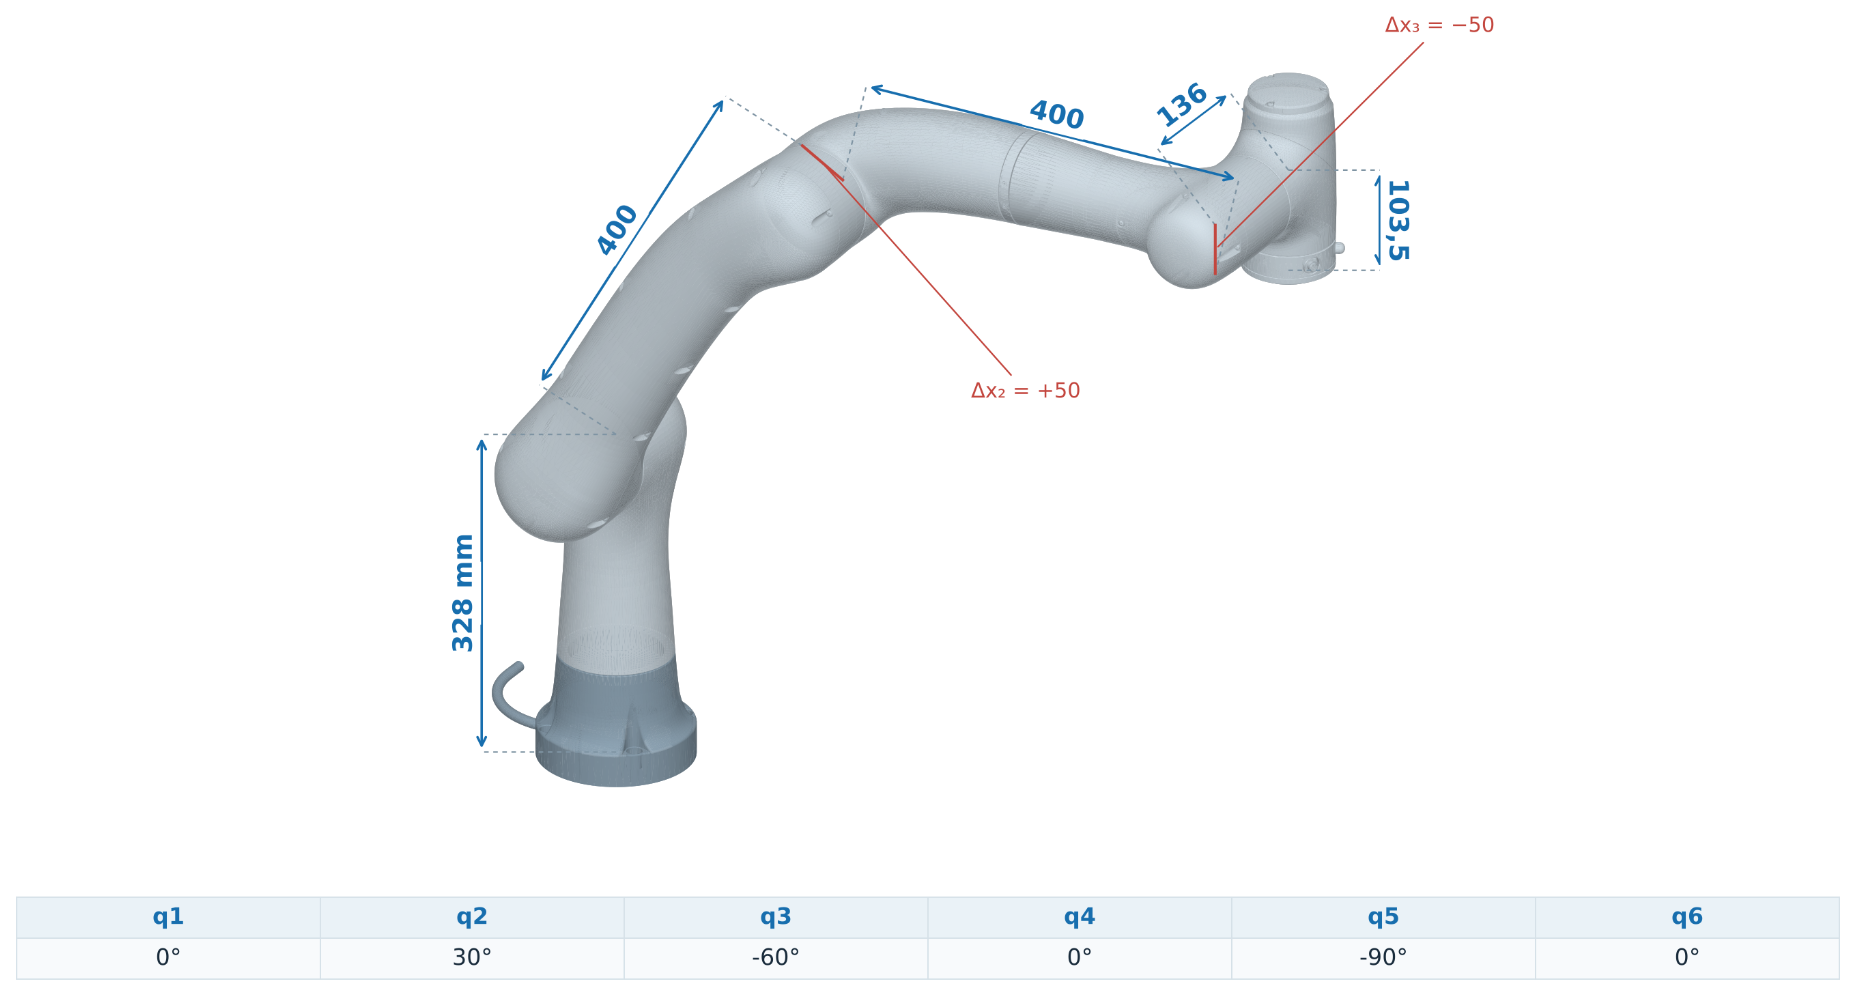
\includegraphics[width=.94\linewidth]{hinh/02-dong-hoc/2.1-cau-tao/hinh-2-1-mo-hinh-sr5.png}
  \caption{Mô phỏng robot ROKAE SR5-5/0.9C}\label{fig:mo-hinh}
\end{figure}

ROKAE SR5-5/0.9C là robot cộng tác thuộc dòng xMate SR, có cấu trúc nối tiếp sáu khớp quay (6R). Tay máy gồm một đế cố định và sáu khâu động, liên kết lần lượt từ đế đến mặt bích lắp dụng cụ. Sáu khớp được ký hiệu từ \(J_1\) đến \(J_6\), tương ứng với sáu biến góc \(\mathbf q=[q_1,q_2,q_3,q_4,q_5,q_6]^{\mathsf T}\). Nhà sản xuất tích hợp cảm biến mômen tại từng khớp để đo mômen tác dụng lên khớp trong quá trình vận hành.

Các bộ phận và thông số hình học được mô tả như sau.
\begin{itemize}
  \item \textbf{Đế và vai.} Trục quay thân \(J_1\) và trục quay vai \(J_2\) vuông góc với nhau. Giao điểm của hai trục nằm ở độ cao \(h\) so với gốc đế.
  \item \textbf{Cánh tay trên.} Từ vai \(J_2\) đến khuỷu \(J_3\), kích thước theo trục \(z_2\) là \(l_1\), độ lệch theo trục \(x_2\) là \(e_1\).
  \item \textbf{Cẳng tay.} Từ khuỷu \(J_3\) đến cổ tay \(J_4\), kích thước theo trục \(z_3\) là \(l_2\), độ lệch theo trục \(x_3\) là \(e_2\).
  \item \textbf{Cổ tay và mặt bích.} Cụm cổ tay gồm ba khớp quay \(J_4,J_5,J_6\). Khoảng cách giữa gốc khớp \(J_4\) và \(J_5\) là \(l_3\). Khoảng cách từ gốc khớp \(J_5\) đến tâm mặt bích lắp dụng cụ là \(l_4\).
  \item \textbf{Bậc tự do và biến khớp.} Robot có sáu bậc tự do. Vị trí và hướng của mặt bích so với đế được xác định từ sáu góc quay trong vectơ \(\mathbf q\).
\end{itemize}
Các kích thước sử dụng trong mô phỏng được lấy từ mô hình xMateSR5 của ROKAE. Theo các trục cục bộ trong mô hình của hãng, các giá trị tính bằng milimét là
\[
\begin{aligned}
h&=328, & l_1&=400, & l_2&=400, & l_3&=136, & l_4&=103{,}5,\\
&&e_1&=50, &e_2&=-50.
\end{aligned}
\]
Do có độ lệch ngang \(50\,\mathrm{mm}\), khoảng cách thẳng từ vai đến khuỷu và từ khuỷu đến cổ tay đều bằng \(\sqrt{400^2+50^2}\approx403{,}1\,\mathrm{mm}\).

\section{Động học robot}
\subsection{Động học thuận robot}
\subsubsection*{Cơ sở lý thuyết của phương pháp Denavit--Hartenberg}
Đối với tay máy nối tiếp, bài toán động học thuận xác định vị trí và hướng của khâu cuối so với đế khi biết các biến khớp. Theo quy ước Denavit--Hartenberg (D--H) chuẩn, ta gắn một hệ tọa độ vào mỗi khâu và mô tả quan hệ giữa hai hệ liên tiếp bằng bốn tham số.

\noindent\textbf{Gán hệ tọa độ.}
Đánh số các khâu từ đế \(\{0\}\) đến khâu cuối \(\{n\}\). Khớp \(i\) nối khâu \(i-1\) với khâu \(i\); trục của khớp này là \(z_{i-1}\). Với hai trục chéo nhau, chọn \(x_i\) dọc theo đường vuông góc chung, từ \(z_{i-1}\) đến \(z_i\). Đường này cắt \(z_{i-1}\) tại \(O'_i\) và cắt \(z_i\) tại gốc \(O_i\). Chọn \(y_i=z_i\times x_i\) để được một hệ thuận tay phải.
\begin{figure}[H]
  \centering
  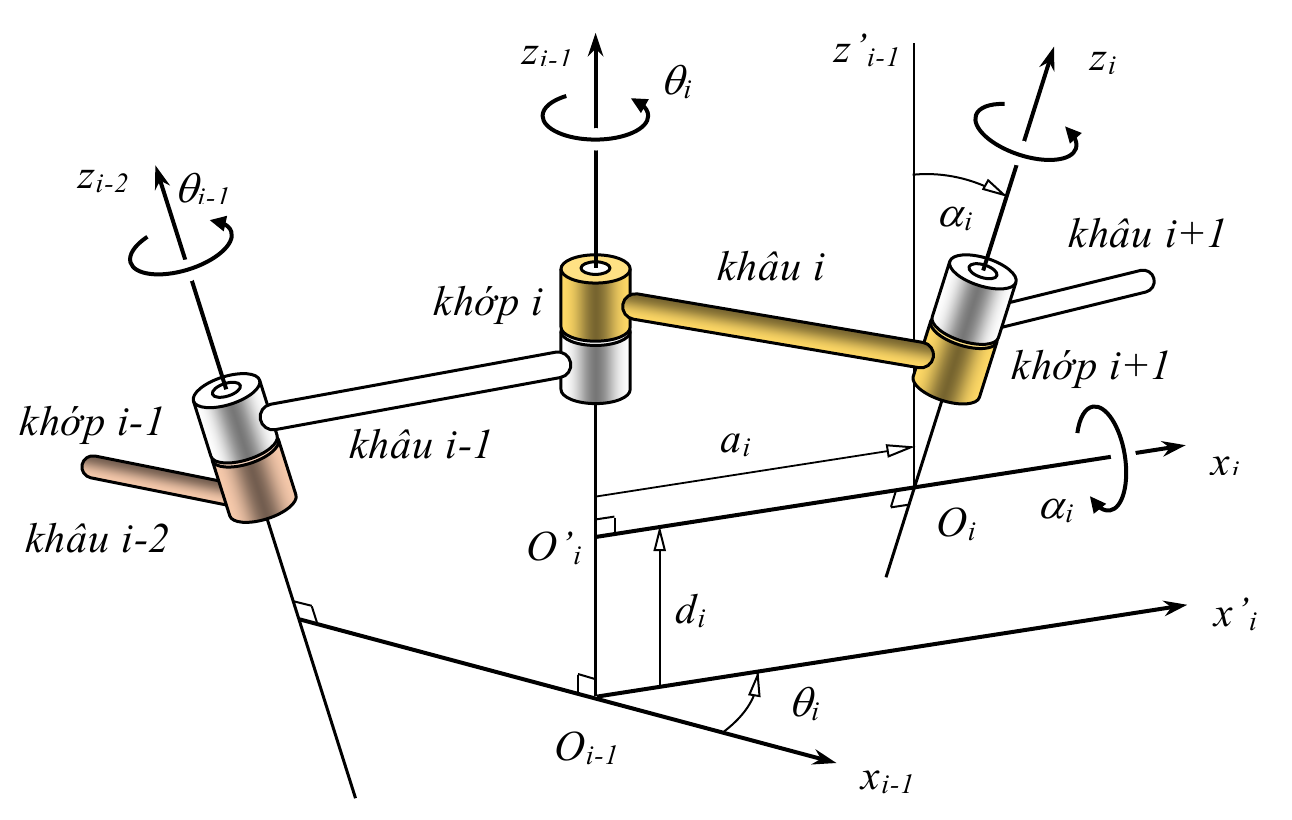
\includegraphics[width=.56\linewidth]{hinh/02-dong-hoc/2.2.1-dong-hoc-thuan/hinh-2-2-quy-uoc-dh.png}
  \caption{Hai hệ trục liên tiếp và bốn tham số D--H. Nguồn: ME3209, hình 3-5, tr.~59.}
  \label{fig:quy-uoc-dh}
\end{figure}

Nếu hai trục khớp song song và phân biệt, có thể chọn vị trí đường vuông góc chung sao cho gốc hệ thuận tiện cho tính toán. Nếu hai trục cắt nhau, đặt gốc tại giao điểm và chọn một trong hai chiều của pháp tuyến làm chiều \(x_i\). Tại đế, có thể chọn \(O_0\) trên \(z_0\) và chọn \(x_0\) vuông góc với \(z_0\). Ở khâu cuối, có thể chọn \(z_n\) song song với \(z_{n-1}\) và chọn \(x_n\) theo quy tắc vuông góc chung. Với khớp tịnh tiến, chiều dương của \(z_{i-1}\) xác định dấu của hành trình.

\noindent\textbf{Ý nghĩa của bốn tham số.}
Hai góc lấy dấu theo quy tắc bàn tay phải quanh trục tương ứng. Hai đoạn tịnh tiến lấy dấu theo chiều dương của trục đo.
\begin{center}
\begin{tabular}{@{}cll@{}}
\toprule
Tham số & Phép đo & Trục dùng để đo\\
\midrule
\(\theta_i\) & Góc quay từ \(x_{i-1}\) đến \(x_i\) & Quanh \(z_{i-1}\)\\
\(d_i\)      & Dịch chuyển từ \(O_{i-1}\) đến \(O'_i\) & Dọc \(z_{i-1}\)\\
\(a_i\)      & Dịch chuyển từ \(O'_i\) đến \(O_i\) & Dọc \(x_i\)\\
\(\alpha_i\) & Góc xoắn từ \(z_{i-1}\) đến \(z_i\) & Quanh \(x_i\)\\
\bottomrule
\end{tabular}
\end{center}
Với khớp quay, \(\theta_i\) thay đổi theo biến khớp \(q_i\), còn \(d_i\) cố định. Với khớp tịnh tiến, \(d_i\) thay đổi, còn \(\theta_i\) cố định. Các tham số \(a_i\) và \(\alpha_i\) đặc trưng cho hình học của khâu.

\noindent\textbf{Biến đổi giữa hai khâu liên tiếp.}
Ký hiệu \({}^{i-1}T_i\) là ma trận đổi tọa độ một điểm từ hệ \(\{i\}\) sang hệ \(\{i-1\}\). Để dựng hệ \(\{i\}\) từ hệ \(\{i-1\}\), lần lượt quay và tịnh tiến theo trục \(z\), rồi tịnh tiến và quay theo trục \(x\) hiện hành. Với vectơ cột, tích tương ứng là
\[
{}^{i-1}T_i=
\operatorname{Rot}_z(\theta_i)\,
\operatorname{Trans}_z(d_i)\,
\operatorname{Trans}_x(a_i)\,
\operatorname{Rot}_x(\alpha_i).
\]
Đặt \(c_\theta=\cos\theta_i,\ s_\theta=\sin\theta_i,\ c_\alpha=\cos\alpha_i,\ s_\alpha=\sin\alpha_i\).
Hai phép biến đổi theo \(z\) cho ma trận bên trái, hai phép theo \(x\) cho ma trận ở giữa. Nhân hai ma trận thu được biểu thức dùng cho từng hàng của bảng D--H:
\[
{}^{i-1}T_i =
\begin{bmatrix}
c_\theta&-s_\theta&0&0\\s_\theta&c_\theta&0&0\\0&0&1&d_i\\0&0&0&1
\end{bmatrix}
\begin{bmatrix}
1&0&0&a_i\\0&c_\alpha&-s_\alpha&0\\0&s_\alpha&c_\alpha&0\\0&0&0&1
\end{bmatrix}
=
\begin{bmatrix}
c_\theta&-s_\theta c_\alpha&s_\theta s_\alpha&a_ic_\theta\\
s_\theta&c_\theta c_\alpha&-c_\theta s_\alpha&a_is_\theta\\
0&s_\alpha&c_\alpha&d_i\\
0&0&0&1
\end{bmatrix}.
\]

\noindent\textbf{Động học thuận của toàn chuỗi.}
Nhân các ma trận theo thứ tự từ đế đến khâu cuối ta được
\[
{}^0T_n(\mathbf q)={}^0T_1(q_1)\,{}^1T_2(q_2)\cdots{}^{n-1}T_n(q_n)
=\begin{bmatrix}{}^0R_n&{}^0\mathbf p_n\\\mathbf 0^{\mathsf T}&1\end{bmatrix}.
\]
Ba cột của \({}^0R_n\) là các vectơ đơn vị của hệ cuối biểu diễn trong hệ đế. Vectơ \({}^0\mathbf p_n\) là tọa độ gốc \(O_n\) trong hệ đế. Với SR5, chuỗi có sáu khớp quay. Khi góc \(q_i\) tăng cùng chiều dương D--H, ta có \(\theta_i=q_i+\theta_{i,0}\), trong đó \(\theta_{i,0}\) là góc đo từ \(x_{i-1}\) đến \(x_i\) khi \(q_i=0\). Đây là cơ sở để xác định các góc lệch cố định trong bảng thông số của SR5.

\subsubsection*{Áp dụng cho robot SR5}
\begin{figure}[H]
  \centering
  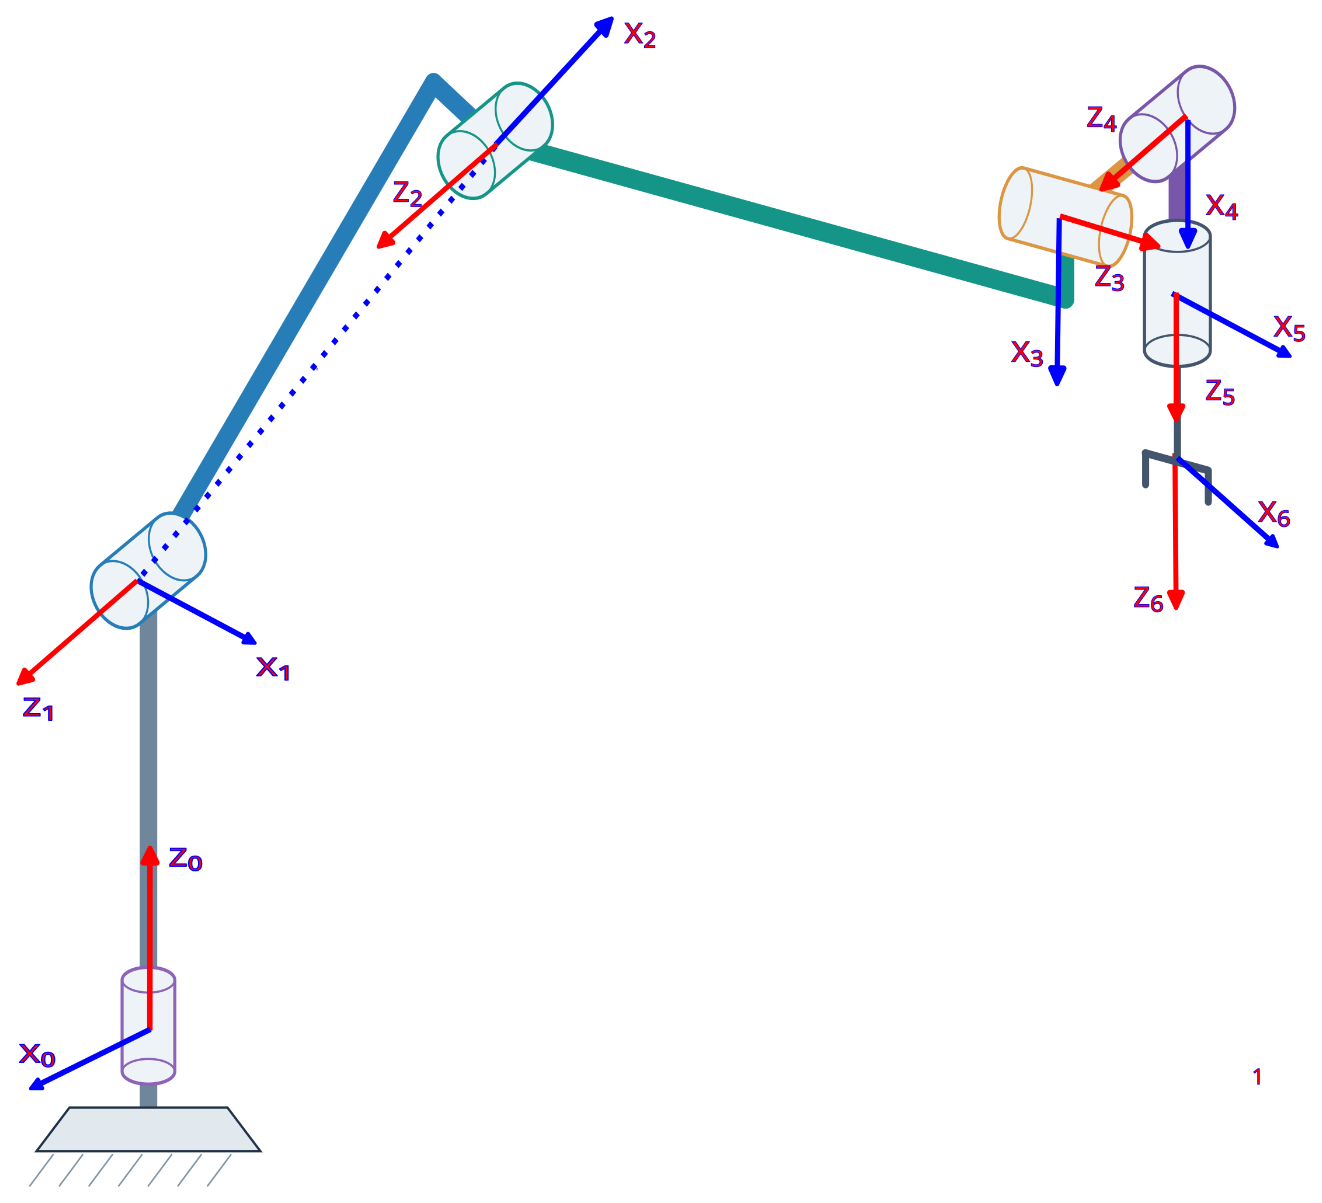
\includegraphics[width=.71\linewidth,height=.35\textheight,keepaspectratio]{hinh/02-dong-hoc/2.2.1-dong-hoc-thuan/hinh-2-3-so-do-khau-khop.png}
  \caption{Sơ đồ khâu, khớp và các trục tọa độ của robot SR5}\label{fig:khau-khop}
\end{figure}

\begin{table}[H]
  \centering
  \caption{Thông số D--H của robot SR5}\label{tab:dh}
  \renewcommand{\arraystretch}{1.12}
  \begin{tabular*}{.80\linewidth}{@{\extracolsep{\fill}}ccccc@{}}
  Khâu \(i\) & \(\theta_i\) & \(d_i\) & \(a_i\) & \(\alpha_i\)\\
  \midrule
  1 & \(q_1\)       & \(d_1\) & 0       & \(\pi/2\)\\
  2 & \(q_2+\beta\) & 0       & \(a_2\) & 0\\
  3 & \(q_3-\beta\) & 0       & \(a_3\) & \(-\pi/2\)\\
  4 & \(q_4\)       & \(d_4\) & 0       & \(\pi/2\)\\
  5 & \(q_5\)       & \(d_5\) & 0       & \(\pi/2\)\\
  6 & \(q_6\)       & \(d_6\) & 0       & 0
  \end{tabular*}
\end{table}
Góc lệch \(\beta=\operatorname{atan2}(400,50)\). Với gốc khớp 1 đặt tại đế, các tham số chiều dài tính bằng milimét là
\[
\begin{aligned}
d_1&=328, & a_2&=\sqrt{400^2+50^2}, & a_3&=-50,\\
d_4&=400, & d_5&=-136, & d_6&=103{,}5.
\end{aligned}
\]
Các góc trong bảng tính bằng radian. Từ bảng thông số D--H, ma trận thuần nhất của hệ cuối so với hệ đế được tính bằng tích
\[
{}^0T_6={}^0T_1\,{}^1T_2\,{}^2T_3\,{}^3T_4\,{}^4T_5\,{}^5T_6.
\]

\subsection{Động học nghịch robot}
\subsubsection*{Cơ sở lý thuyết của bài toán động học nghịch}
\noindent\textbf{Phát biểu tổng quát.}
Theo tài liệu ME3209~\cite[mục 3.2.1, tr.~66--68]{me3209}, cho tư thế đích của khâu cuối
\[
 H=\begin{bmatrix}R_d&\mathbf p_d\\\mathbf 0^{\mathsf T}&1\end{bmatrix}.
\]
Cần tìm \(\mathbf q=[q_1,\ldots,q_n]^{\mathsf T}\) sao cho \(T(\mathbf q)=H\).
So sánh ba hàng đầu của hai ma trận cho 12 phương trình đại số phi tuyến. Ba phần tử của vectơ vị trí và ba tham số độc lập của ma trận quay tạo thành sáu điều kiện tư thế. Bài toán có thể không có nghiệm, có một nghiệm, có nhiều nghiệm rời rạc hoặc có vô số nghiệm, tùy tư thế đích và cấu trúc tay máy. Mỗi nghiệm phải thỏa giới hạn cơ khí \(q_{i,\min}\le q_i\le q_{i,\max}\).

\medskip
\noindent\textbf{Giải bằng phương pháp hình học.}
Dựa vào cấu trúc khâu và trục khớp, chọn các điểm trung gian để rút hệ phương trình tư thế về các quan hệ hình học đơn giản. Nghiệm giải tích cho phép tính trực tiếp biến khớp và liệt kê các nhánh trước khi kiểm tra giới hạn khớp. Khả năng áp dụng phụ thuộc vào cấu trúc tay máy~\cite[mục 3.2.2, tr.~68--70]{me3209}.

Với tay máy phẳng ba khớp quay, gọi \(a_i\) là chiều dài khâu \(i\) và \((x_E,y_E,\phi)\) là tư thế đích. Gốc của khâu cuối nằm tại \(x_B=x_E-a_3\cos\phi\), \(y_B=y_E-a_3\sin\phi\). Áp dụng định lý cosin cho hai khâu đầu, đặt \(D=(x_B^2+y_B^2-a_1^2-a_2^2)/(2a_1a_2)\). Với \(|D|\leq 1\), các góc khớp được tính theo
\begin{align*}
 q_2 &= \operatorname{atan2}\bigl(\pm\sqrt{1-D^2},D\bigr),\\
 q_1 &= \operatorname{atan2}(y_B,x_B)
       -\operatorname{atan2}(a_2\sin q_2,a_1+a_2\cos q_2),\\
 q_3 &= \phi-q_1-q_2 .
\end{align*}
Hai dấu ở căn tạo ra hai nhánh khuỷu khi \(|D|<1\). Tại \(|D|=1\) hai nhánh trùng nhau theo chu kỳ góc. Nếu \(a_1=a_2\) và \(B\) ở gốc, \(q_2=\pi\) theo chu kỳ góc và \(q_1\) không được xác định duy nhất. Nếu \(|D|>1\), điểm \(B\) nằm ngoài miền với tới. Với tay máy tọa độ trụ RTT, các quan hệ \(x_C=q_3\cos q_1\), \(y_C=q_3\sin q_1\), \(z_C=d_1+q_2\) cho \(q_2=z_C-d_1\) và \(q_3=\sqrt{x_C^2+y_C^2}\) khi hành trình hướng kính không âm. Khi đó \(q_1=\operatorname{atan2}(y_C,x_C)\) nếu \(q_3>0\). Nếu cho phép hành trình có dấu, nhánh \(q_3<0\) đi cùng góc \(q_1\) lệch \(\pi\). Khi \(x_C=y_C=0\), vị trí không xác định góc \(q_1\).

\medskip
\noindent\textbf{Giải số bằng phương pháp Newton--Raphson.}
Đặt hệ phương trình phi tuyến \(\mathbf f(\mathbf q)=\mathbf 0\), với \(m\) phương trình và \(n\) biến khớp thực. Ký hiệu \((J_f)_{ab}=\partial f_a/\partial q_b\). Tại vòng lặp \(j\), khai triển Taylor bậc nhất cho
\begin{align*}
 \mathbf f(\mathbf q^{(j)}+\Delta\mathbf q)
 &= \mathbf f(\mathbf q^{(j)})+J_f(\mathbf q^{(j)})\Delta\mathbf q
    + O(\|\Delta\mathbf q\|^2),\\
 J_f(\mathbf q^{(j)})\Delta\mathbf q &=-\mathbf f(\mathbf q^{(j)}),\qquad
 \mathbf q^{(j+1)}=\mathbf q^{(j)}+\Delta\mathbf q .
\end{align*}
Khi \(m=n\) và \(J_f\) khả nghịch, bước lý thuyết là \(\Delta\mathbf q=-J_f^{-1}\mathbf f\). Trình tự lặp theo ME3209~\cite[mục 3.2.3, tr.~71--72]{me3209} gồm:
\begin{enumerate}
  \item Chọn \(\mathbf q^{(0)}\), dung sai \(\varepsilon\) và số vòng lặp tối đa \(M\).
  \item Tính \(\mathbf f(\mathbf q^{(j)})\). Nếu \(\|\mathbf f(\mathbf q^{(j)})\|<\varepsilon\), chấp nhận nghiệm. Nếu đã hết số vòng lặp, kết thúc lần tìm nghiệm.
  \item Tính \(J_f(\mathbf q^{(j)})\), giải hệ tuyến tính tìm \(\Delta\mathbf q\), cập nhật \(\mathbf q^{(j+1)}\) rồi lặp lại.
\end{enumerate}
Có thể theo dõi thêm chuẩn của bước \(\Delta\mathbf q\). Nếu bước nhỏ trong khi sai số vẫn vượt dung sai, nghiệm chưa đạt yêu cầu. Giá trị khởi tạo ảnh hưởng đến khả năng hội tụ và nhánh nghiệm thu được.

\medskip
\noindent\textbf{Chuyển thành bài toán tối ưu có ràng buộc.}
Theo ME3209~\cite[mục 3.2.4, tr.~72--73]{me3209}, có thể tối thiểu hóa sai lệch bình phương giữa các phần tử của ma trận động học thuận và tư thế đích:
\[
 \min_{\mathbf q}\;
 \frac12\sum_{a=1}^{3}\sum_{b=1}^{4}c_{ab}\bigl(T_{ab}(\mathbf q)-H_{ab}\bigr)^2,
 \qquad q_{i,\min}\le q_i\le q_{i,\max}.
\]
Với mọi \(c_{ab}>0\), giá trị mục tiêu bằng không tương ứng với nghiệm tư thế chính xác. Giá trị tối ưu dương cho một tư thế gần đúng và cần được kiểm tra theo dung sai. Khi chỉ yêu cầu vị trí, đặt trọng số của ba cột hướng bằng không. Với tay máy dư dẫn động, có thể bổ sung tiêu chí như giữ khoảng cách tới giới hạn khớp hoặc tránh vật cản.

Ví dụ, với tay máy SCARA, có thể lập hàm mục tiêu từ bốn phần dư tương ứng với ba tọa độ và góc phương vị. Đặt \(q_{12}=q_1+q_2\). Với chiều trục trong ví dụ của ME3209, vectơ phần dư là
\[
 \mathbf f_{\mathrm{SCARA}}=
 \begin{bmatrix}
 a_1\cos q_1+a_2\cos q_{12}-x_C\\
 a_1\sin q_1+a_2\sin q_{12}-y_C\\
 d_1-q_3-d_4-z_C\\
 q_{12}-q_4-\phi
 \end{bmatrix}.
\]
Bài toán là tối thiểu hóa \(\|\mathbf f_{\mathrm{SCARA}}\|^2/2\) trong giới hạn bốn khớp, với phần dư góc được tính theo chu kỳ \(2\pi\).

\medskip
\noindent\textbf{Tách vị trí và hướng.}
Với tay máy sáu khớp có cổ tay cầu, ba trục khớp cuối giao nhau tại tâm cổ tay \(C\). Vị trí điểm này phụ thuộc vào ba khớp đầu. Gọi \({}^{n}\mathbf r_C\) là vectơ từ gốc hệ khâu cuối đến \(C\), biểu diễn trong hệ khâu cuối. Từ tư thế đích, tính
\[
 \mathbf p_C=\mathbf p_d+R_d\,{}^{n}\mathbf r_C
             =\mathbf p_C(q_1,q_2,q_3).
\]
Giải ba phương trình vị trí trước, sau đó giải \({}^3 R_n(q_4,q_5,q_6)=({}^0R_3)^{\mathsf T}R_d\) để tìm các góc cổ tay. Trong ví dụ RTT--RRR của ME3209, \({}^{n}\mathbf r_C=[0,0,-d_6]^{\mathsf T}\) và bài toán vị trí có dạng tọa độ trụ. Phương pháp tách này cần kiểm tra điều kiện hình học của các trục trước khi áp dụng~\cite[mục 3.2.5, tr.~73--75]{me3209}.

\subsubsection*{Thiết lập và giải bài toán động học nghịch cho SR5}
\noindent\textbf{Đặt bài toán.}
Cho trước vị trí \(\mathbf p_{d,k}\) và hướng \(R_{d,k}\) của đầu mỏ hàn tại mẫu \(k\), biểu diễn trong hệ đế \(\{0\}\). Bài toán động học nghịch xác định vectơ góc khớp \(\mathbf q_k=[q_{1,k},\ldots,q_{6,k}]^{\mathsf T}\) sao cho pose của đầu mỏ trùng với pose yêu cầu trong dung sai cho phép. Gọi TCP (Tool Center Point) là điểm làm việc của đầu mỏ. Từ kết quả động học thuận ở mục trước, phương trình cần giải là
\begin{equation}
  {}^0T_{\mathrm{TCP}}(\mathbf q_k)
    = {}^0T_6(\mathbf q_k)\,{}^6T_{\mathrm{TCP}}
    = T_{d,k}, \qquad
  T_{d,k} =
    \begin{bmatrix}
      R_{d,k} & \mathbf p_{d,k}\\
      \mathbf 0^{\mathsf T} & 1
    \end{bmatrix}.
  \label{eq:sr5-ik-pose}
\end{equation}
Ma trận \({}^6T_{\mathrm{TCP}}\) mô tả vị trí và hướng cố định của đầu mỏ trong hệ khâu cuối của bảng D--H. Khi triển khai trong MoveIt~2, chuỗi động học lấy từ URDF và đã chứa khớp cố định nối mặt bích với \textit{welding\_tcp}. Vì vậy, pose đích được truyền trực tiếp cho hệ \textit{welding\_tcp}.

\noindent\textbf{Tuyến tính hóa sai số tư thế TCP.}
Đồ án chọn phương pháp giải số. Phần dư của vị trí là \(\mathbf f_p=\mathbf p(\mathbf q)-\mathbf p_{d,k}\), nên vế phải \(-\mathbf f_p\) là dịch chuyển từ vị trí hiện tại đến vị trí yêu cầu. Với hướng mỏ, KDL dùng vectơ trục--góc của phép quay tương đối làm hiệu chỉnh góc trong hệ đế.

Gọi \(j\) là chỉ số vòng lặp tại mẫu \(k\). Từ bộ góc khớp \(\mathbf q_k^{(j)}\), tính động học thuận để thu được \(\mathbf p^{(j)}\) và \(R^{(j)}\). Sai số pose trong hệ đế được biểu diễn bởi
\begin{equation}
  \mathbf e_k^{(j)} =
    \begin{bmatrix}
      \mathbf p_{d,k}-\mathbf p^{(j)}\\
      \varphi^{(j)}\mathbf u^{(j)}
    \end{bmatrix}.
  \label{eq:sr5-ik-error}
\end{equation}
Trong đó, \(\mathbf u^{(j)}\) và \(\varphi^{(j)}\) lần lượt là trục đơn vị và góc của phép quay \(R_{d,k}(R^{(j)})^{\mathsf T}\). Sai số vị trí tính bằng mét và sai số góc tính bằng radian. Với một biến thiên nhỏ \(\Delta\mathbf q\), ma trận Jacobi hình học tại đầu mỏ cho quan hệ
\[
  J_{\mathrm{TCP}}(\mathbf q_k^{(j)})\,\Delta\mathbf q
    \approx \mathbf e_k^{(j)}.
\]
Công thức lặp cơ bản sử dụng nghịch đảo giả \(J_{\mathrm{TCP}}^+\) để tính bước hiệu chỉnh góc khớp:
\begin{equation}
  \Delta\mathbf q = J_{\mathrm{TCP}}^+\,\mathbf e_k^{(j)},
  \qquad
  \mathbf q_k^{(j+1)}=\mathbf q_k^{(j)}+\Delta\mathbf q.
  \label{eq:sr5-ik-update}
\end{equation}

\noindent\textbf{Bộ giải KDL trong MoveIt~2.}
Plugin \textit{KDLKinematicsPlugin} tính bước hiệu chỉnh bằng phân rã giá trị kỳ dị (SVD). Gọi \(W_x\) và \(W_q\) lần lượt là ma trận trọng số trong không gian thao tác và không gian khớp. Trong một bước giải, bộ giải lập hệ có trọng số và tính
\begin{equation}
  \begin{aligned}
    \widetilde J &= W_xJ_{\mathrm{TCP}}W_q,
    &\widetilde{\mathbf e} &= W_x\mathbf e_k^{(j)},\\
    \widetilde J &= U\Sigma V^{\mathsf T},
    &\Delta\mathbf q &= W_qV\Sigma^+U^{\mathsf T}\widetilde{\mathbf e}.
  \end{aligned}
  \label{eq:sr5-ik-kdl}
\end{equation}
Các phần tử đường chéo của \(\Sigma^+\) bằng \(1/\sigma_i\) đối với các giá trị kỳ dị được giữ lại và bằng \(0\) đối với các giá trị dưới ngưỡng của phép giải SVD. KDL giới hạn bước cập nhật theo giới hạn góc khớp và có thể giảm bước nếu sai số pose tăng. Sau mỗi lần cập nhật, bộ giải tính lại động học thuận. Nghiệm hội tụ khi cả chuẩn sai số vị trí và chuẩn sai số hướng đạt dung sai của bộ giải.

\subsection{Động học vi phân}
\subsubsection*{Công thức tổng quát của ma trận Jacobi}
Xét điểm công tác \(E\) của tay máy chuỗi \(n\) khớp. Gọi \(\mathbf p_E\) và \(R_E\) là vị trí và ma trận quay của hệ dụng cụ đối với hệ đế. Theo ME3209~\cite[mục 3.3.2--3.3.4, tr.~77--87]{me3209}, vận tốc tịnh tiến \(\mathbf v_E\) và vận tốc góc \(\vec{\omega}_E\), biểu diễn trong hệ đế, thỏa mãn
\begin{equation}
  \begin{bmatrix}\mathbf v_E\\\vec{\omega}_E\end{bmatrix}
  =
  \begin{bmatrix}J_v(\mathbf q)\\J_\omega(\mathbf q)\end{bmatrix}
  \dot{\mathbf q}
  =J_E(\mathbf q)\dot{\mathbf q}.
  \label{eq:sr5-velocity-jacobian}
\end{equation}

\noindent\textbf{Tính từ ma trận biến đổi thuần nhất.}
Từ \(\mathbf v_E=\dot{\mathbf p}_E\) suy ra \(J_v=\partial\mathbf p_E/\partial\mathbf q\).
Với ký hiệu \([\mathbf a]_\times\mathbf b=\mathbf a\times\mathbf b\), lấy đạo hàm các cột của \(R_E\) cho \([\vec{\omega}_E]_\times=\dot R_E R_E^{\mathsf T}\). Thay \(\dot R_E=\sum_{i=1}^{n}(\partial R_E/\partial q_i)\dot q_i\) vào công thức này thu được hai khối của cột thứ \(i\):
\[
  J_{v,i}=\frac{\partial\mathbf p_E}{\partial q_i},
  \qquad [J_{\omega,i}]_\times
  =\frac{\partial R_E}{\partial q_i}R_E^{\mathsf T}.
\]

\noindent\textbf{Tính theo phương pháp hình học.}
Gọi \(\mathbf o_{i-1}\) là tọa độ một điểm trên trục khớp \(i\) và \(\mathbf z_{i-1}\) là vectơ đơn vị của trục, cùng biểu diễn trong hệ đế. Khi chỉ khớp quay \(i\) chuyển động, nó tạo vận tốc góc \(\dot q_i\mathbf z_{i-1}\) và vận tốc tịnh tiến tại \(E\) bằng \(\dot q_i\mathbf z_{i-1}\times(\mathbf p_E-\mathbf o_{i-1})\). Khớp trượt tạo vận tốc tịnh tiến \(\dot q_i\mathbf z_{i-1}\) và vận tốc góc bằng không. Cộng đóng góp của từng khớp cho
\begin{equation}
 J_E=[J_{E,1}\ \cdots\ J_{E,n}],\qquad
 J_{E,i}=
 \begin{cases}
  \begin{bmatrix}
   \mathbf z_{i-1}\times(\mathbf p_E-\mathbf o_{i-1})\\
   \mathbf z_{i-1}
  \end{bmatrix}, & \text{khớp quay},\\[8pt]
  \begin{bmatrix}\mathbf z_{i-1}\\\mathbf 0\end{bmatrix}, & \text{khớp trượt}.
 \end{cases}
 \label{eq:sr5-jacobian-column}
\end{equation}
Với một điểm thuộc khâu \(k\), thay \(\mathbf p_E\) bằng vị trí của điểm đó và đặt \(J_{E,i}=\mathbf 0\) cho \(i>k\). Khi đổi cách biểu diễn vận tốc tại cùng điểm \(E\) từ hệ đế sang hệ dụng cụ, nhân cả hai khối của \(J_E\) với \(R_E^{\mathsf T}\).

\noindent\textbf{Quan hệ với Jacobi giải tích.}
Gọi \(\vec{\phi}\) là bộ ba tham số hướng và \(B(\vec{\phi})\) là ma trận thỏa mãn \(\vec{\omega}_E=B(\vec{\phi})\dot{\vec{\phi}}\). Khi \(B\) khả nghịch, Jacobi giải tích là
\[
 J_a=\frac{\partial(\mathbf p_E,\vec{\phi})}{\partial\mathbf q}
     =\begin{bmatrix} I_3&0\\0&B^{-1}(\vec{\phi})\end{bmatrix}J_E.
\]
Với quy ước Euler \(R_E=R_z(\psi)R_x(\theta)R_z(\phi)\), ba cột của \(B\) là các trục quay liên tiếp biểu diễn trong hệ đế:
\[
 \vec{\phi}=[\psi,\theta,\phi]^{\mathsf T},\qquad
 B=\begin{bmatrix}
 0&\cos\psi&\sin\theta\sin\psi\\
 0&\sin\psi&-\sin\theta\cos\psi\\
 1&0&\cos\theta
 \end{bmatrix}.
\]
Với Jacobi hình học, đạo hàm phương trình vận tốc theo thời gian trong hệ đế cho quan hệ gia tốc tổng quát:
\[
 \begin{bmatrix}\mathbf a_E\\\dot{\vec{\omega}}_E\end{bmatrix}
 =J_E\ddot{\mathbf q}+\dot J_E\dot{\mathbf q},
 \qquad
 \dot J_E=\sum_{i=1}^{n}\frac{\partial J_E}{\partial q_i}\dot q_i .
\]

\subsubsection*{Áp dụng cho robot SR5}
Cả sáu cột của \(J_E\) lấy nhánh khớp quay trong phương trình~\eqref{eq:sr5-jacobian-column}. Theo quy ước D--H tiêu chuẩn, trục khớp \(i\) đi qua \(O_{i-1}\) và có hướng \(z_{i-1}\):
\[
 {}^0T_{i-1}=
 \begin{bmatrix}{}^0R_{i-1}&\mathbf o_{i-1}\\\mathbf 0^{\mathsf T}&1\end{bmatrix},
 \qquad
 \mathbf z_{i-1}={}^0R_{i-1}[0,\,0,\,1]^{\mathsf T}.
\]
Với \({}^0T_0=I_4\) và \(\mathbf p_E=[x_E,y_E,z_E]^{\mathsf T}\), cột thứ nhất là
\[
 J_{E,1}=[-y_E,\,x_E,\,0,\,0,\,0,\,1]^{\mathsf T}.
\]
Khi đưa góc khớp từ mô phỏng vào bảng~\ref{tab:dh}, cần quy đổi theo chiều trục của hai mô hình. Gọi \(\mathbf q^{\mathrm{ROS}}\) là góc khớp trong URDF và \(\mathbf q^{\mathrm{DH}}\) là góc dùng trong bảng D--H. Với cách gán hệ hiện tại, chiều dương của khớp 2 và khớp 6 ngược với URDF. Do đó
\[
  S=\operatorname{diag}(1,-1,1,1,1,-1),\qquad
  \mathbf q^{\mathrm{DH}}=S\mathbf q^{\mathrm{ROS}},
  \qquad \dot{\mathbf q}^{\mathrm{DH}}=S\dot{\mathbf q}^{\mathrm{ROS}}.
\]
Hệ 6 trong bảng D--H có trục \(z_6\) ngược chiều trục \(z\) của mặt bích URDF. Từ hệ 6, gốc mặt bích URDF nằm ở tọa độ \(-2d_6=-207\,\mathrm{mm}\) dọc \(z_6\). Trong mô phỏng, TCP nằm thêm \(180\,\mathrm{mm}\) theo chiều dương của trục \(z\) mặt bích. Vì vậy, tọa độ TCP trong hệ 6 là \({}^6\mathbf p_E=[0,\,0,\,-0{,}387]^{\mathsf T}\,\mathrm{m}\). Vị trí cần dùng trong phương trình~\eqref{eq:sr5-jacobian-column} là
\[
  \mathbf p_E=\mathbf o_6+{}^0R_6\,{}^6\mathbf p_E.
\]
Gọi \(J_E^{\mathrm{DH}}\) là ma trận tính theo phương trình~\eqref{eq:sr5-jacobian-column}. Để đối chiếu với MoveIt~2, áp dụng quy tắc dây chuyền cho vận tốc khớp:
\begin{equation}
  J_E^{\mathrm{ROS}}(\mathbf q^{\mathrm{ROS}})
  = J_E^{\mathrm{DH}}(S\mathbf q^{\mathrm{ROS}})\,S.
  \label{eq:sr5-jacobian-ros}
\end{equation}
